% \usepackage{imports}

\begin{figure}[!htb]
\minipage{0.4\textwidth}
    % \tikzset{every picture/.style={line width=0.75pt}} \hspace*{-2.4em}%set default line width to 0.75pt        
    
    \tikzset{every picture/.style={line width=0.75pt}} %set default line width to 0.75pt        
    
    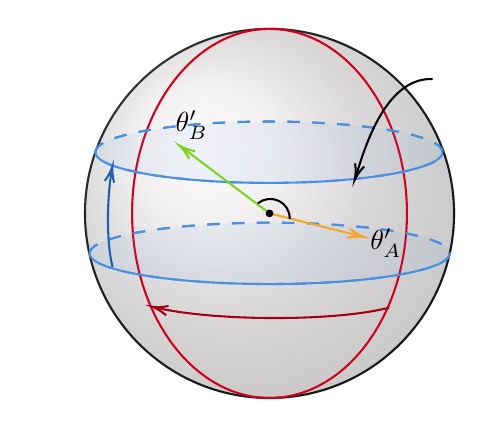
\begin{tikzpicture}[x=0.75pt,y=0.75pt,yscale=-0.7,xscale=0.7]
    %uncomment if require: \path (0,766); %set diagram left start at 0, and has height of 766
    
    %Shape: Circle [id:dp9839498684250778] 
    \draw   (719.4,172) .. controls (719.4,101.86) and (776.26,45) .. (846.4,45) .. controls (916.54,45) and (973.4,101.86) .. (973.4,172) .. controls (973.4,242.14) and (916.54,299) .. (846.4,299) .. controls (776.26,299) and (719.4,242.14) .. (719.4,172) -- cycle ;
    \shade[ball color = gray!40, opacity = 0.3] (846.4,172) circle (3.37cm);
    %Shape: Ellipse [id:dp250735416889859] 
    % \draw  [color={rgb, 255:red, 208; green, 2; blue, 27 }  ,draw opacity=1 ][fill={rgb, 255:red, 208; green, 2; blue, 27 }  ,fill opacity=0.05 ][dash pattern={on 4.5pt off 4.5pt}] (826.15,172) .. controls (826.15,101.86) and (835.22,45) .. (846.4,45) .. controls (857.58,45) and (866.65,101.86) .. (866.65,172) .. controls (866.65,242.14) and (857.58,299) .. (846.4,299) .. controls (835.22,299) and (826.15,242.14) .. (826.15,172) -- cycle ;
    %Shape: Ellipse [id:dp5910425684021126] 
    % \draw  [color={rgb, 255:red, 208; green, 2; blue, 27 }  ,draw opacity=1 ][fill={rgb, 255:red, 208; green, 2; blue, 27 }  ,fill opacity=0.05 ][dash pattern={on 4.5pt off 4.5pt}] (796.41,172) .. controls (796.41,101.86) and (818.79,45) .. (846.4,45) .. controls (874.01,45) and (896.39,101.86) .. (896.39,172) .. controls (896.39,242.14) and (874.01,299) .. (846.4,299) .. controls (818.79,299) and (796.41,242.14) .. (796.41,172) -- cycle ;
    %Shape: Ellipse [id:dp3874552699407441] red lines
    \draw  [color={rgb, 255:red, 208; green, 2; blue, 27 }  ,draw opacity=1 ] [fill={rgb, 255:red, 208; green, 2; blue, 27 }  ,fill opacity=0.01 ](751.81,172) .. controls (751.81,101.86) and (794.16,45) .. (846.4,45) .. controls (898.64,45) and (940.99,101.86) .. (940.99,172) .. controls (940.99,242.14) and (898.64,299) .. (846.4,299) .. controls (794.16,299) and (751.81,242.14) .. (751.81,172) -- cycle ;
    %Shape: Ellipse [id:dp9778496248644617] blue bottom
    \draw  [color={rgb, 255:red, 74; green, 144; blue, 226 }  ,draw opacity=1 ][fill={rgb, 255:red, 74; green, 144; blue, 226 }  ,fill opacity=0.07 ][dash pattern={on 4.5pt off 4.5pt}] (722.5,199.5) .. controls (722.5,187.83) and (778.02,178.37) .. (846.5,178.37) .. controls (914.98,178.37) and (970.5,187.83) .. (970.5,199.5) .. controls (970.5,211.17) and (914.98,220.62) .. (846.5,220.62) .. controls (778.02,220.62) and (722.5,211.17) .. (722.5,199.5) -- cycle ;

    % Front half (top, solid lines)
    \draw  [color={rgb, 255:red, 74; green, 144; blue, 226 }, draw opacity=1 ] (722.5,199.5) .. controls (722.5,211.17) and (778.02,220.62) .. (846.5,220.62) .. controls (914.98,220.62) and (970.5,211.17) .. (970.5,199.5);

    % Back half (top, dashed lines)
    \draw  [color={rgb, 255:red, 74; green, 144; blue, 226 }, draw opacity=1, dash pattern={on 4.5pt off 4.5pt} ] (722.5,199.5) .. controls (722.5,187.83) and (778.02,178.37) .. (846.5,178.37) .. controls (914.98,178.37) and (970.5,187.83) .. (970.5,199.5);
        
    %Shape: Ellipse [id:dp4782644938745719] blue top
    \draw  [color={rgb, 255:red, 74; green, 144; blue, 226 }  ,draw opacity=1 ][fill={rgb, 255:red, 74; green, 144; blue, 226 }  ,fill opacity=0.07 ][dash pattern={on 4.5pt off 4.5pt}] (726.5,129.87) .. controls (726.5,118.21) and (780,108.75) .. (846,108.75) .. controls (912,108.75) and (965.5,118.21) .. (965.5,129.87) .. controls (965.5,141.54) and (912,151) .. (846,151) .. controls (780,151) and (726.5,141.54) .. (726.5,129.87) -- cycle ;

    % Front half (bottom, solid lines)
    \draw  [color={rgb, 255:red, 74; green, 144; blue, 226 }, draw opacity=1 ] (726.5,129.87) .. controls (726.5,141.54) and (780,151) .. (846,151) .. controls (912,151) and (965.5,141.54) .. (965.5,129.87);
    
    % Back half (top, dashed lines)
    \draw  [color={rgb, 255:red, 74; green, 144; blue, 226 }, draw opacity=1, dash pattern={on 4.5pt off 4.5pt} ] (726.5,129.87) .. controls (726.5,118.21) and (780,108.75) .. (846,108.75) .. controls (912,108.75) and (965.5,118.21) .. (965.5,129.87);
    
    %Curve Lines [id:da7445805344753933] 
    \draw [color={rgb, 255:red, 165; green, 0; blue, 20 }  ,draw opacity=1 ]   (928.83,236.83) .. controls (890.75,246.68) and (806.74,246.18) .. (767.27,236.61) ;
    \draw [shift={(765.5,236.17)}, rotate = 14.5] [color={rgb, 255:red, 165; green, 0; blue, 20 }  ,draw opacity=1 ][line width=0.75]    (10.93,-3.29) .. controls (6.95,-1.4) and (3.31,-0.3) .. (0,0) .. controls (3.31,0.3) and (6.95,1.4) .. (10.93,3.29)   ;
    %Straight Lines [id:da5634336743977284] 
    \draw [color={rgb, 255:red, 126; green, 211; blue, 33 }  ,draw opacity=1 ][fill={rgb, 255:red, 65; green, 117; blue, 5 }  ,fill opacity=1 ]   (846.4,172) -- (786,126.45) ;
    \draw [shift={(784.4,125.25)}, rotate = 37.02] [color={rgb, 255:red, 126; green, 211; blue, 33 }  ,draw opacity=1 ][line width=0.75]    (10.93,-3.29) .. controls (6.95,-1.4) and (3.31,-0.3) .. (0,0) .. controls (3.31,0.3) and (6.95,1.4) .. (10.93,3.29)   ;
    %Straight Lines [id:da3395546173482795] 
    \draw [color={rgb, 255:red, 245; green, 166; blue, 35 }  ,draw opacity=1 ]   (846.4,172) -- (909.46,187.76) ;
    \draw [shift={(911.4,188.25)}, rotate = 194.04] [color={rgb, 255:red, 245; green, 166; blue, 35 }  ,draw opacity=1 ][line width=0.75]    (10.93,-3.29) .. controls (6.95,-1.4) and (3.31,-0.3) .. (0,0) .. controls (3.31,0.3) and (6.95,1.4) .. (10.93,3.29)   ;
    %Curve Lines [id:da9757293733184289] 
    \draw    (958.67,79.5) .. controls (925.21,78.21) and (911.01,130.16) .. (905.56,147.28) ;
    \draw [shift={(905,149)}, rotate = 288.43] [color={rgb, 255:red, 0; green, 0; blue, 0 }  ][line width=0.75]    (10.93,-3.29) .. controls (6.95,-1.4) and (3.31,-0.3) .. (0,0) .. controls (3.31,0.3) and (6.95,1.4) .. (10.93,3.29)   ;
    %Shape: Arc [id:dp5356965422841637] 
    \draw  [draw opacity=0] (838.37,165.05) .. controls (842.13,161.98) and (847.53,161.11) .. (852.36,163.25) .. controls (857.52,165.54) and (860.55,170.6) .. (860.41,175.79) -- (847.03,175.22) -- cycle ; \draw   (838.37,165.05) .. controls (842.13,161.98) and (847.53,161.11) .. (852.36,163.25) .. controls (857.52,165.54) and (860.55,170.6) .. (860.41,175.79) ;  
    %Curve Lines [id:da5925626178256742] 
    \draw [color={rgb, 255:red, 29; green, 95; blue, 173 }  ,draw opacity=1 ]   (738.33,208.83) .. controls (733.81,190.08) and (734.61,159.88) .. (738.01,141.2) ;
    \draw [shift={(738.33,139.5)}, rotate = 101.21] [color={rgb, 255:red, 29; green, 95; blue, 173 }  ,draw opacity=1 ][line width=0.75]    (10.93,-3.29) .. controls (6.95,-1.4) and (3.31,-0.3) .. (0,0) .. controls (3.31,0.3) and (6.95,1.4) .. (10.93,3.29)   ;
    
    % Text Node
    \draw (966.33,58.5) node [anchor=north west][inner sep=0.75pt]   [align=left] {$\IsoPL{\bB}$};
    % Text Node
    \draw (863,156.17) node [anchor=north west][inner sep=0.75pt]   [align=left] {$\dvAng$};
    % Text Node
    \draw (779.67,99.17) node [anchor=north west][inner sep=0.75pt]   [align=left] {$\theta_B'$};
    % Text Node
    \draw (913.67,180.5) node [anchor=north west][inner sep=0.75pt]   [align=left] {$\theta_A'$};
    % Text Node
    \draw (680.67,158.17) node [anchor=north west][inner sep=0.75pt]   [align=left] {};
    % Text Node
    \draw (867.67,249.17) node [anchor=north west][inner sep=0.75pt]   [align=left] {$\IsoPL{\aB}$};
    
    \fill[fill=black] (846.4,172) circle (2pt);
    \end{tikzpicture}
    \caption{Illustration of isoplanar subspaces for players A and B.} \label{fig:isoplane}
\endminipage\hfill
\minipage{0.4\textwidth}
    \tikzset{every picture/.style={line width=0.75pt}} %set default line width to 0.75pt        
    
    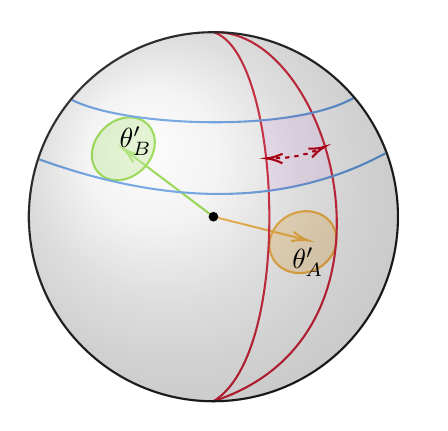
\begin{tikzpicture}[x=0.75pt,y=0.75pt,yscale=-0.7,xscale=0.7]
    %uncomment if require: \path (0,766); %set diagram left start at 0, and has height of 766
    
    %Straight Lines [id:da6265083795426538] 
    \draw [color={rgb, 255:red, 126; green, 211; blue, 33 }  ,draw opacity=1 ][fill={rgb, 255:red, 65; green, 117; blue, 5 }  ,fill opacity=1 ]   (494.4,164) -- (434,118.45) ;
    \draw [shift={(432.4,117.25)}, rotate = 37.02] [color={rgb, 255:red, 126; green, 211; blue, 33 }  ,draw opacity=1 ][line width=0.75]    (10.93,-3.29) .. controls (6.95,-1.4) and (3.31,-0.3) .. (0,0) .. controls (3.31,0.3) and (6.95,1.4) .. (10.93,3.29)   ;
    %Straight Lines [id:da11805825679548954] 
    \draw [color={rgb, 255:red, 245; green, 166; blue, 35 }  ,draw opacity=1 ]   (494.4,164) -- (557.46,179.76) ;
    \draw [shift={(559.4,180.25)}, rotate = 194.04] [color={rgb, 255:red, 245; green, 166; blue, 35 }  ,draw opacity=1 ][line width=0.75]    (10.93,-3.29) .. controls (6.95,-1.4) and (3.31,-0.3) .. (0,0) .. controls (3.31,0.3) and (6.95,1.4) .. (10.93,3.29)   ;
    %Shape: Ellipse [id:dp7609292848935025] 
    \draw  [color={rgb, 255:red, 245; green, 166; blue, 35 }  ,draw opacity=1 ] [fill={rgb, 255:red, 245; green, 166; blue, 35 }  ,fill opacity=0.3 ] (534.06,177) .. controls (537.96,165.49) and (550.94,158.18) .. (563.06,160.67) .. controls (575.18,163.15) and (581.84,174.49) .. (577.94,186) .. controls (574.04,197.51) and (561.06,204.82) .. (548.94,202.33) .. controls (536.82,199.85) and (530.16,188.51) .. (534.06,177) -- cycle ;
    %Shape: Ellipse [id:dp46179464913124435] 
    \draw  [color={rgb, 255:red, 126; green, 211; blue, 33 }  ,draw opacity=1 ] [fill={rgb, 255:red, 184; green, 233; blue, 134 }  ,fill opacity=0.47 ] (413.44,110.89) .. controls (419.21,99.47) and (432.38,93.05) .. (442.86,96.56) .. controls (453.33,100.07) and (457.14,112.18) .. (451.36,123.61) .. controls (445.59,135.03) and (432.42,141.45) .. (421.94,137.94) .. controls (411.47,134.43) and (407.66,122.32) .. (413.44,110.89) -- cycle ;
    %Curve Lines [id:da7557709955412175] 
    % [dash pattern={on 4.5pt off 4.5pt}]
    \draw [color={rgb, 255:red, 208; green, 2; blue, 27 }  ,draw opacity=1 ]   (494.4,37) .. controls (540.8,50.6) and (550.4,257.4) .. (494.4,291) ;
    %Curve Lines [id:da49920065304717465] 
    \draw [color={rgb, 255:red, 208; green, 2; blue, 27 }  ,draw opacity=1 ]  (494.4,37) .. controls (575.2,34.6) and (636,245) .. (494.4,291) ;
    %Curve Lines [id:da2841718150567425] 
    \draw [color={rgb, 255:red, 74; green, 144; blue, 226 }  ,draw opacity=1 ]  (374.5,124.5) .. controls (461.1,155.9) and (543.1,158) .. (612.7,120.4) ;
    %Curve Lines [id:da2808434295323503] 
    \draw [color={rgb, 255:red, 74; green, 144; blue, 226 }  ,draw opacity=1 ]  (397,83.6) .. controls (433,102) and (548.2,106.7) .. (591.4,82) ;
    %Shape: Polygon [id:ds7620014830782629] 
    \draw  [draw opacity=0][fill={rgb, 255:red, 189; green, 16; blue, 224 }  ,fill opacity=0.09 ] (527.67,97.83) -- (546.33,95.17) -- (562.33,92.5) -- (571,115.83) -- (576.33,135.83) -- (555.67,141.83) -- (533,146.5) -- (531,123.83) -- cycle ;
    %Shape: Circle [id:dp81886672741732] 
    \draw   (367.4,164) .. controls (367.4,93.86) and (424.26,37) .. (494.4,37) .. controls (564.54,37) and (621.4,93.86) .. (621.4,164) .. controls (621.4,234.14) and (564.54,291) .. (494.4,291) .. controls (424.26,291) and (367.4,234.14) .. (367.4,164) -- cycle ;
    \shade[ball color = gray!40, opacity = 0.3] (494.4,164) circle (3.37cm);
    %Curve Lines [id:da6392617087009791] 
    \draw [color={rgb, 255:red, 165; green, 0; blue, 20 }  ,draw opacity=1 ] [dash pattern={on 0.84pt off 2.51pt}]  (571,115.83) .. controls (562.84,120.79) and (548.69,123.76) .. (532.97,123.84) ;
    \draw [shift={(531,123.83)}, rotate = 0.58] [color={rgb, 255:red, 165; green, 0; blue, 20 }  ,draw opacity=1 ][line width=0.75]    (10.93,-3.29) .. controls (6.95,-1.4) and (3.31,-0.3) .. (0,0) .. controls (3.31,0.3) and (6.95,1.4) .. (10.93,3.29)   ;
    %Curve Lines [id:da4888688530956691] 
    \draw [color={rgb, 255:red, 165; green, 0; blue, 20 }  ,draw opacity=1 ] [dash pattern={on 0.84pt off 2.51pt}]  (531,123.83) .. controls (547.71,123.99) and (557.13,121.72) .. (569.27,116.58) ;
    \draw [shift={(571,115.83)}, rotate = 156.45] [color={rgb, 255:red, 165; green, 0; blue, 20 }  ,draw opacity=1 ][line width=0.75]    (10.93,-3.29) .. controls (6.95,-1.4) and (3.31,-0.3) .. (0,0) .. controls (3.31,0.3) and (6.95,1.4) .. (10.93,3.29)   ;
    
    % Text Node
    \draw (427.67,100.17) node [anchor=north west][inner sep=0.75pt]   [align=left] {$\theta_B'$};
    % Text Node
    \draw (546.67,183.5) node [anchor=north west][inner sep=0.75pt]   [align=left] {$\theta_A'$};
    % Text Node
    \draw (536.33,85.17) node [anchor=north west][inner sep=0.75pt]   [align=left] {$\IsoPL{\aB}$};

    \fill[fill=black] (494.4,164) circle (2.5pt);
    \end{tikzpicture}
    \caption{Illustration of geodesic confidence balls for players A and B.} \label{fig:conf-ball}
\endminipage\hfill
\caption*{\textbf{Diagram Description:} A visualization of the isoplanes $\IsoPL{\aB}$ and $\IsoPL{\bB}$ on a 2-sphere embedded in three dimensions is shown in Fig. \ref{fig:isoplane}. The isoplanes are depicted relative to the normalized objective vectors $\theta_A'$ and $\theta_B'$, which lie on the manifold surface, separated by a divergence angle $\alpha_{Div}$. Figure \ref{fig:conf-ball} illustrates the geodesic confidence balls, positioned on the surface of the spherical manifold. In three dimensions, it becomes evident that $\IsoPL{\aB}$ and $\IsoPL{\bB}$ are orthogonal at any point of intersection. This intersection, denoted by $\IsoPL{\bB_{\aB}}$, is where the joint action emerges, represented by a purple geodesic square indicating the uncertainty region.} 
\end{figure}

% \begin{tikzpicture}
%   \shade[ball color = gray!40, opacity = 0.4] (0,0) circle (2cm);
%   \draw (0,0) circle (2cm);
%   \draw (-2,0) arc (180:360:2 and 0.6);
%   %\draw[dashed] (2,0) arc (0:180:2 and 0.6);
%   \fill[fill=black] (0,0) circle (1pt);
%   %\draw[dashed] (0,0 ) -- node[above]{$r$} (2,0);
% \end{tikzpicture}